\documentclass[11pt]{article}
\usepackage[utf8]{inputenc}
\usepackage{mathtools}
\usepackage{vmargin}
\usepackage{graphicx}
\usepackage{lmodern}
\usepackage[T1]{fontenc}
\usepackage{multirow}
\usepackage[noline,ruled,linesnumbered,spanish]{algorithm2e}
\usepackage{forest}
\usepackage{forest,adjustbox}
\usepackage{color}

\setpapersize{A4}
\setmargins{2.5cm}       % margen izquierdo
{0cm}                        % margen superior
{16.5cm}                      % anchura del texto
{23.42cm}                    % altura del texto
{10pt}                           % altura de los encabezados
{1cm}                           % espacio entre el texto y los encabezados
{0pt}                             % altura del pie de página
{2cm}                           % espacio entre el texto y el pie de página

\title{Mini-Proyecto III: Estructuras de Datos Sucintas}
\author{Cristobal Donoso Oliva}
\author{
Diego Seco$^{1}$, Meraioth Ulloa Salazar$^{2}$, Cristóbal Donoso Oliva$^{3}$,\\ Matías Medina Silva$^{4}$,\\ \\
\small{$^{1}$Docente a cargo de la asignatura$^{2-3-4}$Estudiantes Pre-grado}\\
\small{$^{1-2}$Dpto. de Ingeniería Civil Informática y Ciencias de la Computación}\\
\small{Universidad de Concepción, Concepción, Chile.}\\
}
\date{Noviembre de 2016}
\usepackage{amsmath}
\begin{document}

\maketitle

\section{Range Minimum Query}
\subsection{Descripción del Problema}
El problema de RMQ (Range Minimum Query) consiste en encontrar el mínimo dentro de un rango [i,j] perteneciente a un arreglo de n objetos que se pueden comparar. En particular, resolveremos el problema para un arreglo de números. Usualmente debemos resolver RMQ en el desarrollo de otros problemas, tales como: Lowest Common Ancestors o del áres de Document Retrieval.
\begin{center}\begin{tabular}{|c|c|c|c|c|c|c|}
\hline
	13 & 2 & 7 & 0 & 9 & 10 & 27 \\
\hline
\end{tabular}
\\\scriptsize{\color{white}.\color{black}\\Figura 1: Data set con números}
\end{center}
Sea $RMQ$ la función que retorna el minimo del rango $[i,j]$, con 0$\le$i$\le$ j$\le$n, entonces: \begin{center}$RMQ[2,6] = 0$\\$RMQ[0,2] = 2$\\$RMQ[4,4] = 9$\end{center}  
En la práctica existen varias soluciones candidatas a este problema, sin embargo, no todas ellas rinden de igual manera. Con el objetivo de comparar experimentalmente la complejidad asociada al RMQ, \emph{utilizaremos dos implementaciones básicas y una estructura de datos sucinta}.

\subsection{Solución Naive}
Consiste en almacenar los mínimos asociados a todas las sub-cadenas que pertenecen al arreglo de números; con esto realizamos consultas en tiempo $O(1)$, sin embargo, la complejidad espacial asciende a $O(n^2)$. Cabe mencionar que en situaciones donde \emph{el recurso espacial no es relevante}, implementar esta solución es una alternativa rápida y sencilla a la hora de computar las consultas, sin embargo, es importante añadir que los datos consultados deben cumplir la condición de \emph{ser estáticos}, en su defecto, el dinamismo actualizaría la tabla frecuentemente aumentando el tiempo de pre-procesamiento.\\\\A continuación se muestra la matriz resultante del set de números propuesto anteriormente(ver figura 1).
\begin{center}$\begin{vmatrix}
	13 & 2 & 2 & 0 & 0 & 0 & 0 \\
	 & 2 & 2 & 0 & 0 & 0 & 0 \\
	 &  & 7 & 0 & 0 & 0 & 0 \\
	 &  &  & 0 & 0 & 0 & 0 \\
	 &  &  &  & 9 & 9 & 9 \\
	 &  &  &  &  & 10 & 27 \\
	 &  &  &  &  &  & 27 \\
\end{vmatrix}$
\\\scriptsize{\color{white}.\color{black}\\Figura 2: Matriz que guarda los mínimos parciales de todos los rangos de un conjunto de números}
\end{center}
Una consulta simple bastaría con preguntar por la dirección $<i,j>$ de la matriz generada.

\subsection{Solución RMQ + Sparse Table}
Podemos resolver el problema RMQ optimizando la matriz que almacena los mínimos utilizando potencias de dos para definir la dimensión de la tabla (sparse table). Esta alternativa nos permite disminuir el espacio realizando consultas en tiempo constante. En efecto, las complejidades asociadas al espacio y consulta son $O(nlog(n))$ y $O(1)$ respectivamente.\\\\La cantidad de filas corresponden a los datos en el set, sin embargo, las columnas responden a $O(log(n))$. La idea consiste en pre-computar el mínimo de todas las sub-cadenas de tamaño $2^k$ donde $0 \le k \le log(n)$. Del mismo set (figura 1) la tabla generada es:

\begin{center}$\begin{vmatrix}
	0 & 1 & 3   \\
	1 & 1 & 3   \\
	2 & 3 & 3   \\
	3 & 3 &     \\
	4 & 4 &     \\
	5 & 5 &     \\
	6 &   &	    \\
\end{vmatrix}$
\\\scriptsize{\color{white}.\color{black}\\Figura 2: Sparse Table para el set}
\end{center}
Para calcular la tabla es necesario saber la cantidad de columnas $j$ que tendrá la tabla, para ello calculamos:
\begin{center}$\#j$ = log(\emph{$\#$ elementos})  $\iff \lfloor log(7) \rfloor+1 \iff 2 +1 = 3$
\end{center}
Donde $\#$ representa la cardinalidad y $log$ es de base 2. Luego buscamos los mínimos que se encuentran dentro de los rangos $2^j$ con $0\le j \le 2$ para cada posición $i$. Para realizar la consulta debemos comparar:
\begin{center}$arr[lookup[i][j-1]]$ $\nabla$ $arr[lookup[i+2^j-1-1][j-1]]$\end{center}
Donde $\nabla$ = $\{\le,\geq\}$. RMQ retorna el menor entre los valores comparados. 

\subsection{Solución RMQ Succinct}
RMQ Succinct es, teóricamente, la mejor alternativa a la hora de computar las busquedas de un mínimo dentro de un set. Esta solución utiliza la técnica de Indirección con el objetivo de simplificar aún más la complejidad asociada al espacio.\\\\La idea consiste en generar $\frac{2n}{log(n)}$ bloques de tamaño $\frac{1}{2}log(n)$ e ir guardando resúmenes en cada nivel de manera que acceder a los datos mínimos sea muy rápido.  
\begin{figure}[htp]
\centering
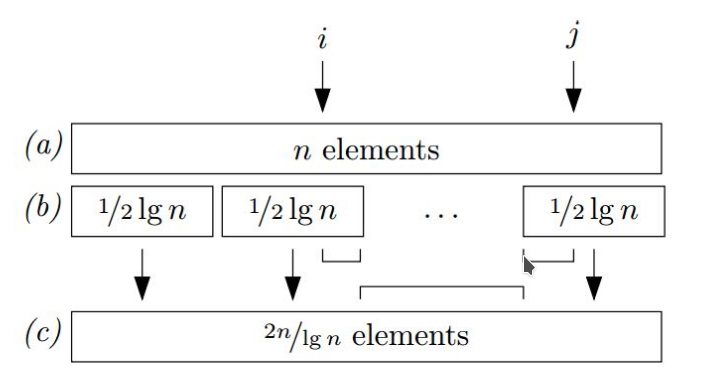
\includegraphics[scale=0.5]{indirecion.png}
\\\scriptsize{\color{white}.\color{black}\\Figura 3: Representación gráfica de los bloques generados en un modelo de indirección}
\label{}
\end{figure}
Con todo esto logramos obtener espacio $O(n)$ y $O(1)$ consulta.\\\\En la práctica utilizaremos la librería SDSL (https://github.com/simongog/sdsl-lite) la cual trae implementado un RMQ sucinto. Haremos uso de del método \textbf{rmq} de la clase \emph{rmq\_succinct\_sct} al cual le pasamos como parámetros los límites del rango a considerar.
\subsection{Experimento y Resultados}
Anteriormente determinamos teóricamente la complejidad espacial de los tres algoritmos en cuestión. Es fácil demostrar en la práctica como influye la construcción de las tablas ya que éstas alteran la tiempo de ejecución en directa proporción con la cantidad de elementos. En ese sentido, al realizar consultas bajo \emph{datasets} espacialmente dinámicos, las soluciones deberían diferir bastante entre sí.\begin{center}\emph{\textbf{Hipótesis}\\Para un vector de tamaño variable y que almcaena número la alternativa Sucinta saca ventaja en tiempo a los otras alternativas.}\end{center}Para realizar los experimentos se utilizó un procesador \emph{AMD Phenom(tm) 9550 Quad-Core Processor} y se dispuso de 8GB de RAM. \\\\Para los \emph{sets aleatorios} de tamaño $10^i$ con 0<i<$10^7$ y rango $[0,random(0...i)]$ se obtuvieron los siguientes resultados:
\begin{center}\begin{tabular}{|l|c|c|c|}
\hline
	$Tamaño$ & $Naive$ & $Sparse$ & $Succinct$\\
\hline
	10       & 7.7e-5   & 4.4e-5      & 2.4e-05\\
\hline
	100 	 & 0.002429 & 0.000441    & 4.7e-05 \\
\hline
	1000     & 0.097398 & 0.004381    & 0.000217\\
\hline
	10000    & 8.8443   & 0.031585    & 0.00169\\
\hline
	100000   & killed   & 0.0323302   & 0.003774\\
\hline
	1000000  & killed   & 3.63675     & 0.034628\\
\hline
	10000000 & killed   & 40.3935     & 0.349027\\
\hline
\end{tabular}
\\\scriptsize{\color{white}.\color{black}\\Figura 4: Tabla de resultados tiempo de ejecución algoritmos propuestos}
\end{center}
Para mayor claridad solo se muestra el gráfico hasta i = 800 puesto que las rectas difieren mucho producto del orden de complejidad.
\begin{center}\begin{figure}[htp]
\centering
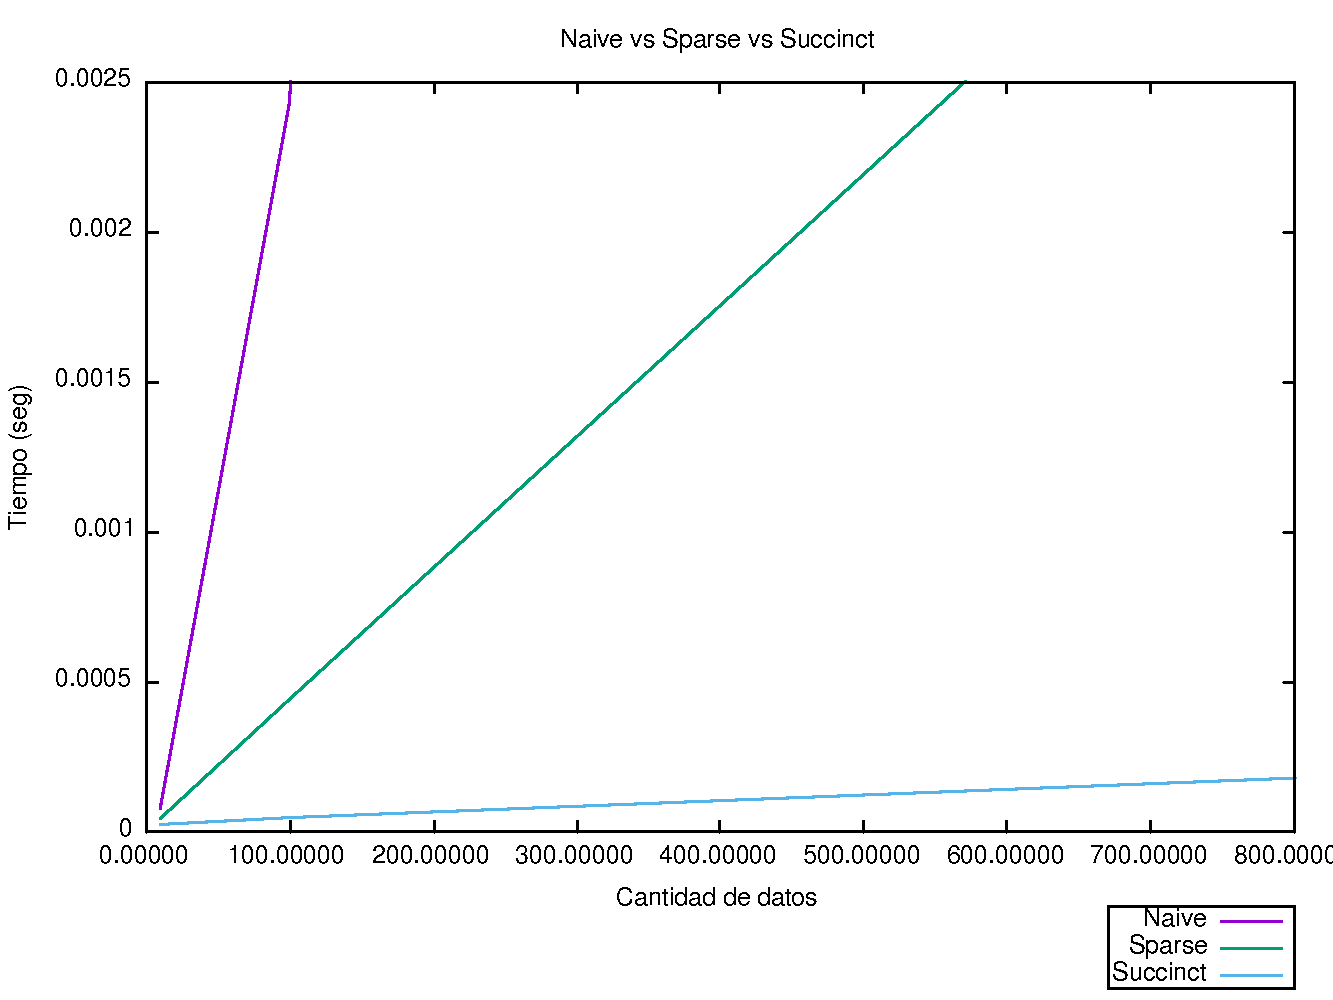
\includegraphics[scale=0.6]{grafico.pdf}
\\\scriptsize{\color{white}.\color{black}\\Figura 5: Bifurcación que muestra las diferencias en tiempo de ejecución de los algoritmos naive y sparse}
\label{etiqueta}
\end{figure}
\end{center}
Se puede apreciar como la alternativa sucinta saca ventaja de su compresión. A raíz de los resultados empíricos es posible reconocer cuales son las mejores alternativas. En el caso particular de la solución Naive, vemos como se dispara de manera cuadrática la curva. En escenarios donde no importa el recurso memoria naive se podría utilizar, sin embargo, la mayoría de los problemas actuales necesitan manejo de grandes volúmenes de datos. Sparse significa una simplificación importante y podría ser útil para volúmenes de hasta $10^5$ datos, consideramos más fácil de implementar que una estructura de datos sucinta.Aún cuando los recursos sean abundantes y la dificultad del código no sea problema, tratamos de buscar la alternativa más rápida y de menor espacio (considerando que todos los recursos son escasos y debemos optimizarlos).
\section{predecesor y sucesor}
\subsection{Descripción del problema}
Se tiene \textbf{t} elementos de un conjunto [1,n] y se quieren hacer dos tipos de consultas sobre dicho conjunto:
\begin{itemize}
\item Sucesor: Dado un número i, ¿Cuál es el menor número $\geq$ i en el conjunto?
\item Predecesor: Dado un número i, ¿Cuál es el mayor número $\leq$ i en el conjunto?
\end{itemize}
Para este problema se proponen dos soluciones usando las siguientes estructuras de datos:
\subsection{Solución BST}
Para poder calcular el predecesor y sucesor de un elemento del BST primero debemos definir el mínimo y máximo elemento en un árbol binario. Los nodos mínimo y máximo de un BST se encontrarían más a la izquierda y más a la derecha respectivamente desde la raíz (ver figura 6 y 7). 
\begin{figure}[htp]
\centering
\begin{minipage}{.4\textwidth}
\centering
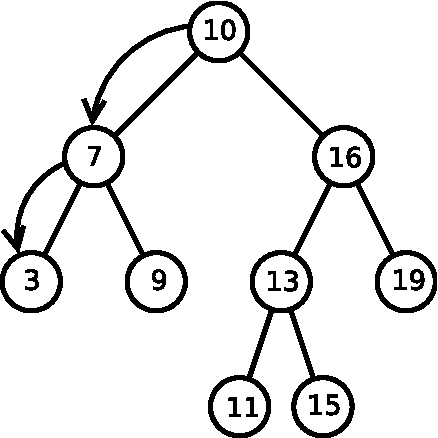
\includegraphics[scale=0.5]{min_arbol.pdf}
\\\scriptsize{\color{white}.\color{black}\\Figura 6: Nodo mínimo en un BST}
\label{etiqueta}
\end{minipage}
\begin{minipage}{.4\textwidth}
\centering
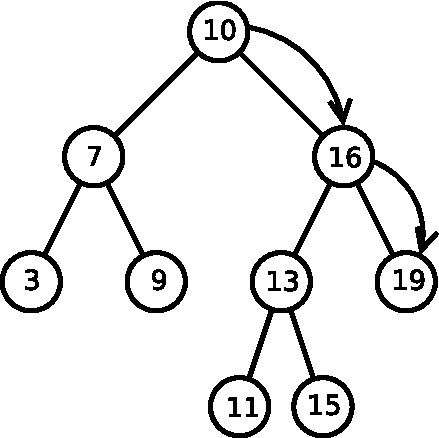
\includegraphics[scale=0.5]{max_arbol.pdf}
\\\scriptsize{\color{white}.\color{black}\\Figura 7: Nodo máximo en un BST}
\label{etiqueta}
\end{minipage}
\end{figure}

Entonces, Para poder encontrar el predecesor y sucesor:
\begin{itemize}
\item Si el nodo i tiene dos hijos su predecesor es el valor máximo en el sub-árbol a la izquierda de i y su sucesor sería el valor mínimo en en el sub-árbol a la derecha de i.
\item Si no entonces:
\begin{itemize}
\item Si i no tiene hijo izquierdo entonces su predecesor es su primer ancestro izquierdo.
\item Si i no tiene hijo derecho entonces su sucesor es su primer ancestro derecho.
\end{itemize}
\end{itemize}
\subsection{Solución Bitmap}
Cada indice del bitmap B representa un elemento de conjunto [1,n], donde un 1 representa que el elemento es uno de los t elementos, como se puede ver en la figura 8.\\

\begin{figure}[htp]
\centering
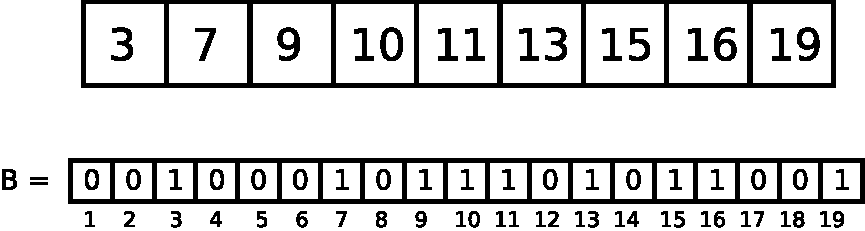
\includegraphics[scale=0.5]{bitmap.pdf}
\\\scriptsize{\color{white}.\color{black}\\Figura 8: Nodo mínimo en un BST}
\end{figure}
Para responder a las consultas predecesor y sucesor podemos usar las operaciones rank y select de los bitmaps:
\begin{itemize}
\item Sucesor: Select(B, Rank (B, i) + 1)
\begin{figure}[htp]
\centering
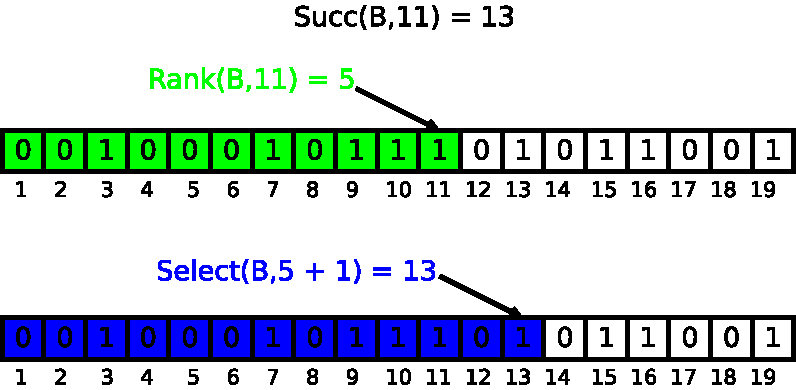
\includegraphics[scale=0.5]{bitmapsuc.pdf}
\\\scriptsize{\color{white}.\color{black}\\Figura 9: Ejemplo de sucesor con i = 11}
\end{figure}
\item Predecesor: Select(B, Rank (B, i $-$ 1))
\begin{figure}[htp]
\centering
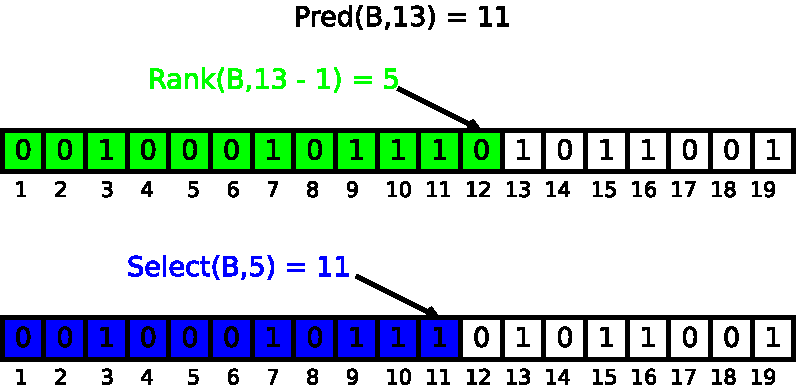
\includegraphics[scale=0.5]{bitmappred.pdf}
\\\scriptsize{\color{white}.\color{black}\\Figura 10: Ejemplo de predecesor con i = 11}
\end{figure}
\end{itemize}
\subsection{Análisis de complejidad de las soluciones}
\subsubsection{BST}
Las operaciones necesarias para obtener el predecesor y sucesor toman un tiempo que es proporcional a la altura del árbol. Para un BST con n nodos, las operaciones quedan acotadas a tiempos O(Log(n)) usando el método de análisis en el caso promedio y acotadas a tiempos O(n) usando el método de peor caso, cuando el árbol no está balanceado y hay que recorrer los nodos de manera secuencial.
\subsubsection{Bitmap}
Las únicas operaciones utilizadas en el bitmap son rank y select, las cuales pueden ser respondidas en tiempo constante O(1) utilizando bitmaps normales y también en tiempo O(k) para rank (k es la clave) y O(log n)  para select utilizando bitmaps H$_{0}$ - comprimidos, ambos ya implementados en la librería sdsl.
\subsection{Implementación de soluciones}
Se implementaron 3 clases en c++, BinarySearchTree, BitMap y BitMapH0, cada una de estas clases recibe como parámetro en su método constructor un vector de datos y a partir de este se inicializa cada estructura con dichos datos.

\subsubsection{BinarySearchTree}
Correspondiente a los archivos bst.cpp y bst.h, esta clase se implementó a partir de nodos que contienen un dato y punteros a sus hijos izquierdo, derecho y su nodo padre. La clase tiene guardada el nodo raíz y a partir del mismo se localiza el resto de los nodos.
\subsubsection{BitMap}
Corrrespondiente a los archivos bitmap.cpp y bitmap.h, esta clase se implementó a partir de la clase bit$\_$vector de la librería sdsl. La clase contiene un bit$\_$vector el cual tiene soporte de rank y select, métodos utilizados para obtener el predecesor y sucesor.
\subsubsection{BitMapH0}
Correspondiente a los archivos bitmap$\_$h0.cpp y bitmap$\_$h0.h, esta clase se implementó a partir de la clase rrr$\_$vector de la librería sdsl. Dicha clase corresponde a un bitmap H$_{0}$-comprimido y también tiene soporte de rank y select, ambos métodos utilizados de la misma forma que para BitMap, se podría decir que ambas clases son análogas.
\subsection{Dataset para los experimentos}
Para poder medir el tiempo de ejecutar la operación predecesor y sucesor, se utilizó un vector con \textbf{M} datos no repetidos, ordenados randómicamente en un rango \textbf{[1,N]}, con M = N / 2 en cada iteración. El valor de \textbf{M} disminuye a la mitad por cada iteración en un total de 8 iteraciones. El tamaño inicial del vector es de 8 Mb, siendo este incrementado hasta 1 Gb. Se utilizó el mismo vector para cada clase por iteración, solo cambiando este al comenzar una nueva iteración.
\subsection{Resultados experimentales}
\subsubsection{Formulación de hipótesis}
En base al análisis de complejidad de cada solución en el caso promedio, el bitmap debería ser más rápido, seguido por bitmap H$_{0}$-comprimido y finalmente el bst. 
\subsubsection{Experimento}
El siguiente experimento fué ejecutado en un computador con un procesador Intel Core i5 3230M (2600 MHz - 3200 MHz) con 12 Gb de memoria RAM. En cada iteración se ejecutó cada operación (predecesor y sucesor) 10.000 veces por cada clase sobre un elemento randómico distinto contenido en el vector original. Se midió el tiempo por cada operación y se calculó un promedió de las 10.000 operaciones distintas por cada clase.
\subsubsection{Resultados}
Luego de finalizada la ejecución del experimento se obtuvieron los siguientes resultados, con M medido en Mb y el tiempo promedio de cada operación medido en mili segundos.
\begin{center}\begin{tabular}{|l|c|c|c|c|c|c|}
\hline
	$M$ & $BST$ $pred$ & $BST$ $suc$ & $BM$ $pred$ & $BM$ $suc$ & $BMH_{0}$ $pred$ & $BMH_{0}$ $suc$ \\
\hline
8	&   1.3475	&   1.3522	&   0.4340 &	   0.4316 &	   1.0165 &	   0.9804 \\
\hline
16	&   1.3773	&   1.3798	&   0.4331 &	   0.4364 &	   0.9887 &	   0.9636 \\
\hline
32	&   1.6508	&   1.6432	&   0.4608 &	   0.4638 &	   1.0265 &	   0.9989 \\
\hline
64	&   1.9108	&   1.8856	&   0.5019 &	   0.5050 &	   1.0507 &	   1.0301 \\
\hline
128	 &  2.1253	&   2.1073	&   0.5466 &	   0.5527 &	   1.0985 &	   1.0647 \\
\hline
256	 &  2.3634	&   2.3445	&   0.5784 &	   0.5686 &	   1.2045 &	   1.1638 \\
\hline
512	 &  2.8431	&   2.8241	&   0.6605 &	   0.6470 &	   1.3886 &	   1.3410 \\
\hline
1024 &	   2.9252	&   2.9399	&   0.6229 &	   0.6148 &	   1.2804 &	   1.2132 \\ 
\hline
\end{tabular}
\\\scriptsize{\color{white}.\color{black}\\Figura 11: Tabla de resultados tiempo de ejecución algoritmos propuestos}
\end{center}
Para mejor visualización y análisis, se graficó los datos de la figura 11 en dos gráficos, uno para sucesor y otro para predecesor.
\begin{center}\begin{figure}[htp]
\centering
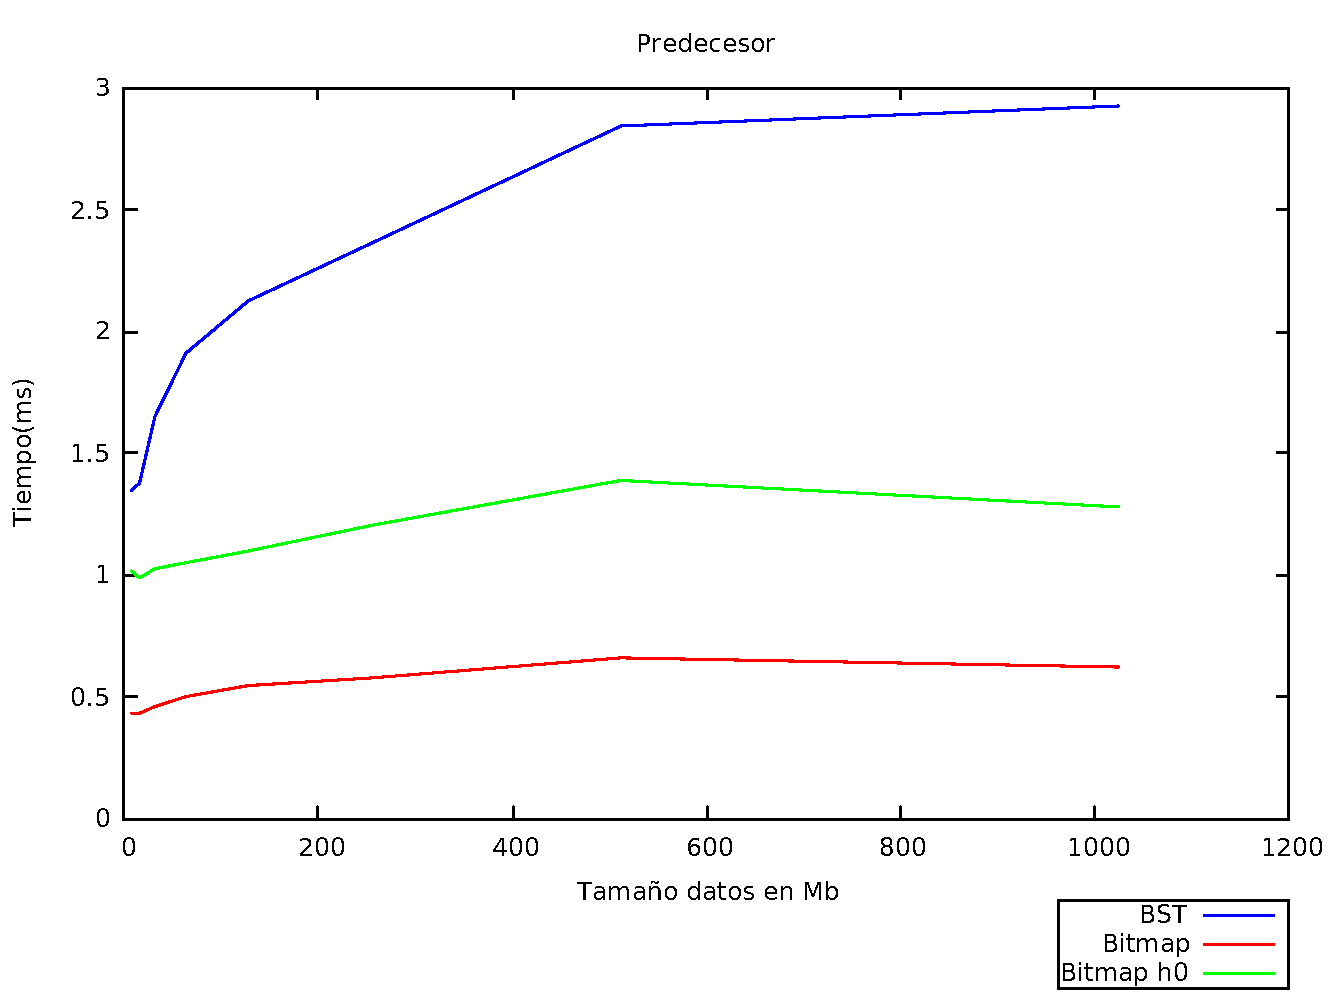
\includegraphics[scale=0.45]{exppred.pdf}
\\\scriptsize{\color{white}.\color{black}\\Figura 12: Comparación de soluciones para predecesor}
\label{etiqueta}
\end{figure}
\end{center}
\begin{center}\begin{figure}[htp]
\centering
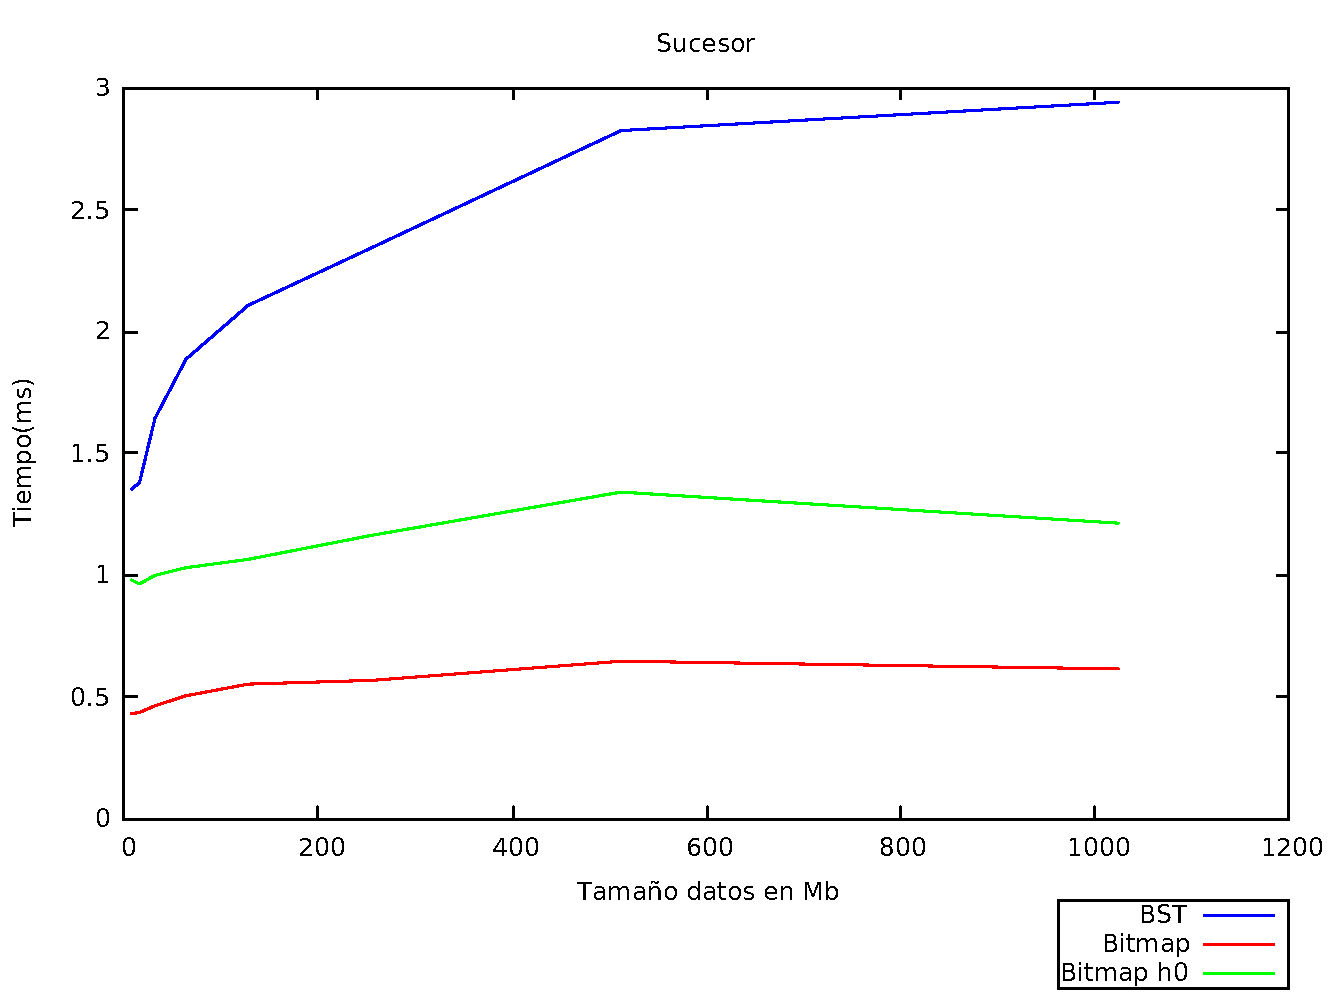
\includegraphics[scale=0.45]{expsuc.pdf}
\\\scriptsize{\color{white}.\color{black}\\Figura 13: Comparación de soluciones para sucesor}
\label{etiqueta}
\end{figure}
\end{center}
\clearpage
\subsubsection{Conclusión experimento}
Como podemos ver en la figura 11 y 12, los resultados obtenidos comprueban la hipótesis formulada al comienzo del experimento, para el cálculo del predecesor y sucesor el peor resultado obtenido fue la solución del BST. la curva de este tiene forma logarítmica. Para los bitmaps, el bitmap sin compresión obtuvo el mejor resultado.\\

Para el problema de predecesor y sucesor, la utilización de bitmaps presentó una mejora sobre el uso de binary search tree en términos de tiempo y espacio. El bitmap sin compresión es más rápido que su contraparte comprimida pero, evidentemente, gasta más espacio, por lo tanto la utilización de uno sobre otro depende de los requerimientos, si se debe priorizar tiempo por sobre espacio entonces es recomendable utilizar bitmap sin compresión, en el caso contrario es mejor utilizar bitmap H$_{0}$-comprimido.

\section{Perfect Hashing}
\subsection{Descripción del Problema}
Una función hash es cualquier función , que pueda ser usada para mapear un dato
(objeto , string , etc.) de tamaño variable , a un dato de tamaño fijo. El valor retornado por la función hash , suele llamarse hash value o hash code.


El problema consiste en satisfacer la necesidad de mapear datos de tamaño variable a datos de tamaño fijo, y realizar consultas de elementos en tiempo constante O(1),en la solución comunmente utilizada ( unordered\_map) aun usando diversas funciones hash, existe la posibilidad de que ocurran colisiones ( Cuando datos distintos obtienen el mismo hash value), pudiendo manejarlas al menos de dos maneras , Open Addressing y Separate Chaining , que nos llevan a soluciones que no son O(1) en peor caso.


Nuestro objetivo en este trabajo es mostrar que con el uso de bitmaps y la operación rank sobre los bitmap , se puede mantener una funcion hash perfecta , es decir con tiempo constante para consultar por algun elemento en el conjunto, contrarestando con una estructura de común uso para el mismo problema, unordered\_map. 
\subsection{Preeliminar}

Se define:
\begin{enumerate}
    \item Key: Valor a mapear, en específico para este trabajos el dominio serán los enteros.
    \item Value: Dato que es guardado en la posición a la que fue mapeado Key.
    \item n : Valor máximo de Key posible, es decir cualquier Key estará en el intervalo [1, ... , n]
    \item t : Cantidad de elementos, que serán mapeados.
    \item r : Número de bits para representar el dato a guardar ( Value).
\end{enumerate}
\\
Para efectos de este trabajo, se realizarán las siguientes asunciones:
\begin{enumerate}
    \item El conjunto de Key se encuentra ordenado, en una etapa de preprocesamiento, con una priority queue , con un costo total de O(t*log(t)), donde t es la cantidad de elementos.
    \item r será la cantidad necesaria para representar entero , es decir 32 bits.
\end{enumerate}
\\
Para esta implementación se hizo uso de la librería SDSL-lite ( de estructuras sucintas), las estructuras sucintas son representaciones de objetos ( vectores, arboles, etc) ocupando un espacio cercano al limite inferior teorico ( según teoría de información) soportando operaciones de las estructuras originales en tiempo eficiente. 
\\
En específico se hizo uso de bitvector, que es un array de bits es decir en cada posicion del arreglo solo pueden haber dos valores posibles, 1 ó 0, esta estructura sucinta ocupa espacio $O(64[n/64+1])$, tambien se usó la clase $rank\_support\_v$, es una estructura que implementa la operacion rank sobre un bitvector (la operación rank cuenta la cantidad de 1 que existen hasta la posicion i-esima) ocupa un espacio adicional de $O(0.25n)$ y resuelve la operacion rank en tiempo de ejecución $O(1)$.


\subsection{Solución}
Teniendo una estructura que soporta rank sobre un bitvector se procede de la siguiente forma para un arreglo de enteros A de t elementos , y un bitmap B de n elementos:

\begin{center}\begin{tabular}{|c|c|c|c|c|c|c|}
\hline
	2 & 4 & 7 & 10 & 11 & 12 & 17 \\
\hline
\end{tabular}

\\\scriptsize{\color{white}.\color{black}\\Figura x: Representación del arreglo A, cada elemeno es una Key}
\end{center}
\begin{center}
\begin{enumerate}
    \item Se itera sobre el arreglo A que contiene todas las Keys. 
    \item Por cada Key , se marca en el bitmap un 1 en la posición $Key$ de bitmap.
    
\end{enumerate}
\\
\begin{tabular}{|c|c|c|c|c|c|c|c|c|c|c|c|c|c|c|c|c|c|}
\hline
	 0 & 1 & 0 &1 &0 &0 &1 &0 & 0 & 1 & 1 & 1 & 0 & 0 & 0 & 0 & 1 &0 \\
\hline
\end{tabular}
\\\scriptsize{\color{white}.\color{black}\\Figura x: Representación de un bitmap B, cada elemento es un 1 o 0}
\end{center}

Ahora para consultar si alguna Key i existe, basta con consultar primero si $B[i]==1$, si es asi , accedemos al value de la key i de la forma: $A[rank_B(i)]$ .
\begin{center}\begin{figure}[htp]
\centering
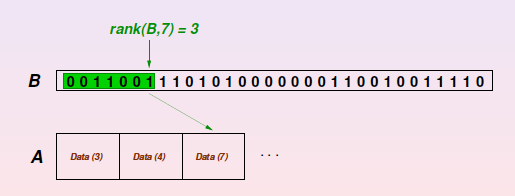
\includegraphics[scale=0.5]{3.png}
\\\scriptsize{\color{white}.\color{black}\\Figura Z:Acceder al elemento i en el arreglo A  }
\label{etiqueta}
\end{figure}
\end{center}


Cabe destacar que esta técnica de perfect hashing fue aplicada en un contexto estatico, es decir asumimos que tenemos un arreglo ordenado por Key de menor a mayor por lo cual no es incluido el pre-procesamiento del arreglo en el analisis de tiempo.
\subsection{Hipotesis}
Para efectos de este trabajo, se considero $r$ como la cantidad de bits para representar un entero. 
\\
Nuestras hipotesis antes de ejecutar los experimentos son:
\begin{enumerate}
    \item La solución implementando bitvector y rank ocupa menos espacio que unordered\_map.
    \item La solución implementando bitvector y rank tiene mejor tiempo de ejecución debido a que asegura consultas en tiempo constante.
    \item Podrian obtenerse mejores resultados en cuanto a espacio concierne, disminuyendo la cantidad de bits para representar los datos value.
\end{enumerate}


\subsection{Análisis de tiempo}
Para nuestras soluciones al problema los analisis de tiempo serán solo para encontrar alguna Key (existente o no, dentro de bitvector y unordered\_map) son:
\begin{enumerate}
    \item Solucion array A+bitvector+rank : O(1) Peor caso
    \item Solucion unordered\_map : O(1) Caso promedio, O(n) en peor caso,con n tamaño del contenedor.
\end{enumerate}
\\

\subsection{Experimentos}
Para los experimentos, se fijo un n (tamaño máximo de key) en 100000.
Aumentando a cantidad de elementos o Keys hasta llegar al maximo.

\begin{center}\begin{figure}[htp]
\centering
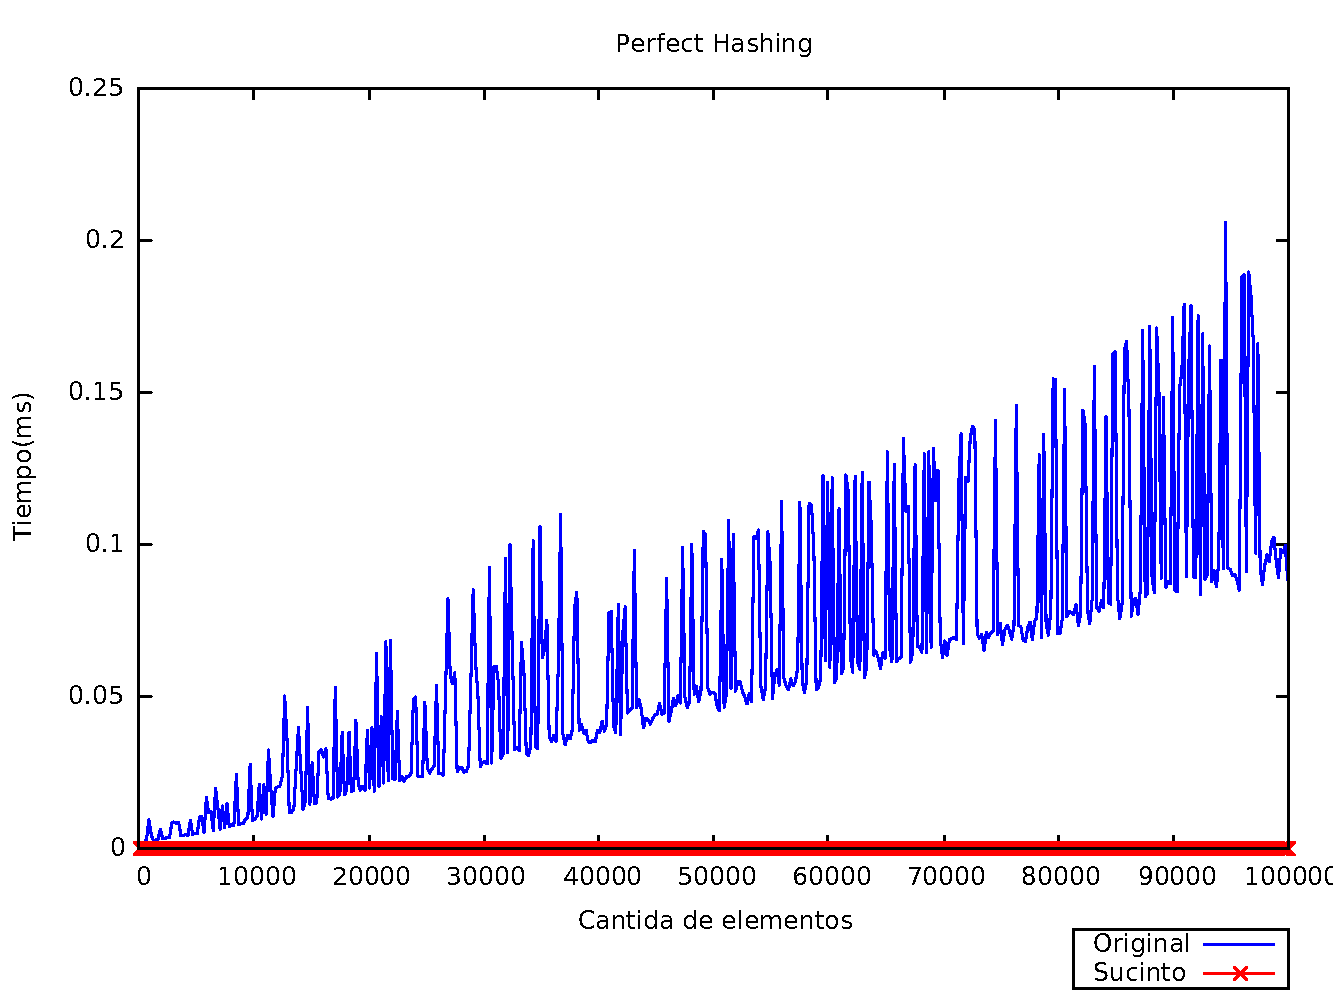
\includegraphics[scale=0.5]{1.pdf}
\\
\scriptsize{\color{white}.\color{black}\\Figura Z:Grafica Cantidad elementos vs Tiempo }
\label{etiqueta}
\end{figure}
\end{center}


\begin{center}\begin{figure}[htp]
\centering
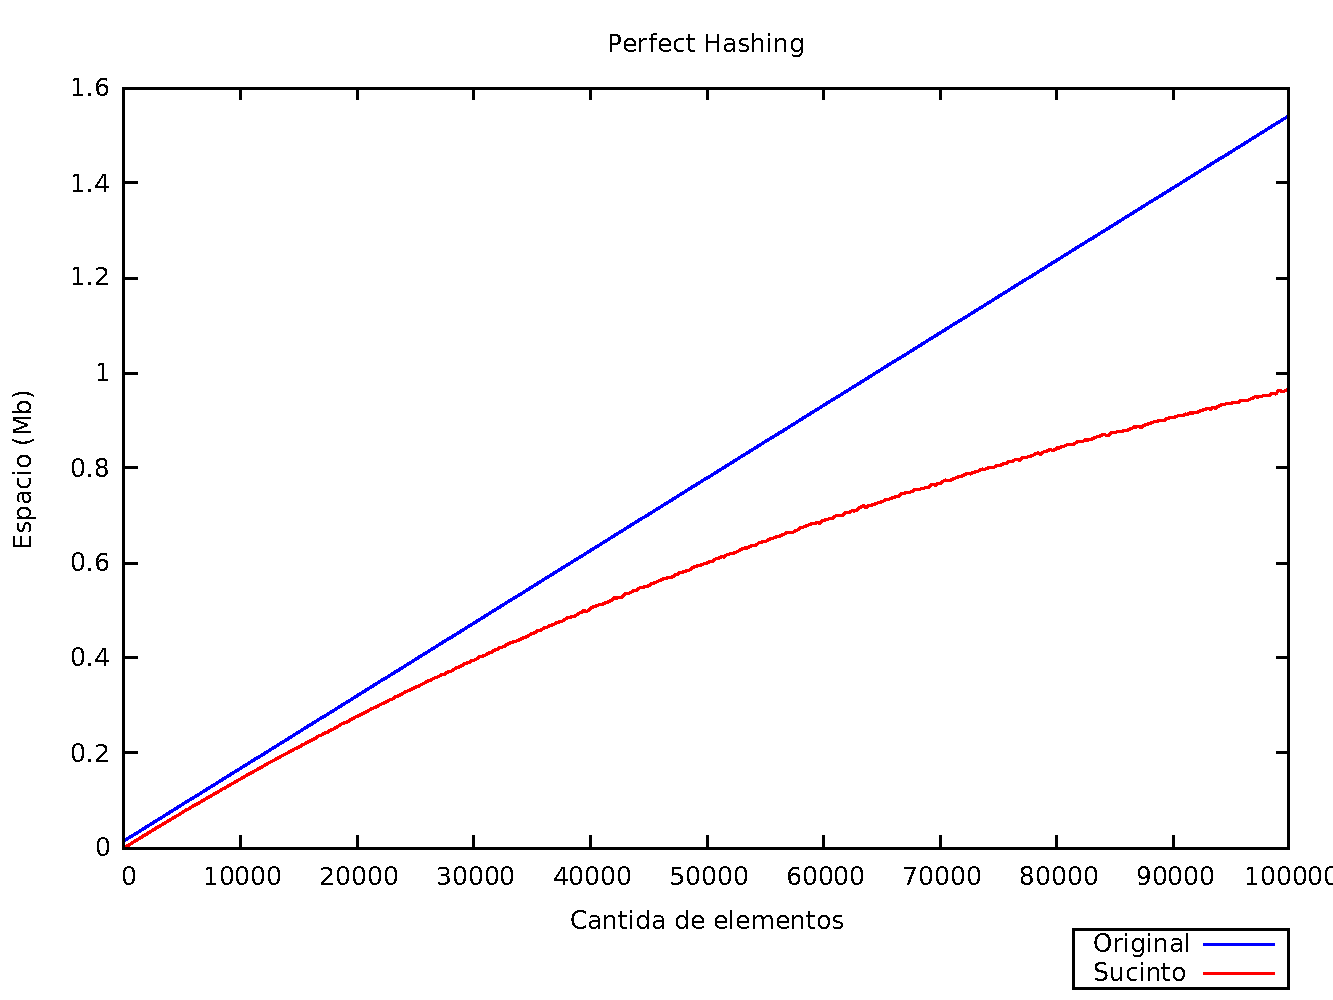
\includegraphics[scale=0.5]{2.pdf}
\\
\scriptsize{\color{white}.\color{black}\\Figura Z:Grafica Cantidad elementos vs Tiempo }
\label{etiqueta}
\end{figure}
\end{center}
\subsection{Conclusiones}

Se concluye que bajo las hipotesis propuestas :
\begin{enumerate}
    \item Efectivamente nuestra solución implementada con bitvector y rank, tienen un comportamiento constante.
    \item La solución implementando bitvector y rank debido a que son estructuras compactas ocupan menos espacio , notar que el parecido en las graficas , es por causa del arreglo de datos ( en nuestro caso enteros) A.
    \item Si tuvieramos conocimiento del dominio es especifico podriamos representar en menos bits los datos y asi disminuir aun mas la brecha de espacio.
    \item Cuando la relacion $t/n$ es muy pequeña (menor a 0,1) ocupar cualquier solucion es indiferente para un analisis de espacio.
\end{enumerate}
\end{document}
